\chapter{The LinqToWiki library}

The LinqToWiki library consists of one Visual Studio solution, that contains the following projects:

\begin{itemize}
\item LinqToWiki.Core
\item LinqToWiki.Codegen
\item LinqToWiki.Codegen.App
\item LinqToWiki.ManuallyGenerated
\item LinqToWiki.Samples
\end{itemize}

The LinqToWiki.Core project contains the core of the library:
types that access the API, convert to and from the representation of data in the API,
represent parameters of various types of queries, represent query results
or those that process LINQ expression trees.
This project can be used together with code generated using LinqToWiki.Codegen,
or with manually written code.

The LinqToWiki.Codegen project handles generating code based on information from the \texttt{paraminfo} module.
It contains types that represent the results of that module, process them, generate C\# code and compile this code using Roslyn.
This project also contains helper types for easier creating of Roslyn syntax trees.

The LinqToWiki.Codegen.App compiles down to a simple console application called linqtowiki-codegen,
that uses the functionality from the LinqToWiki.\allowbreak{}Codegen project.

The LinqToWiki.ManuallyGenerated project is a sample of how one could write code to access a wiki using LiqToWiki without using LinqToWiki.Codegen to generate the code.

Finally, the LinqToWiki.Samples project contains samples showing how to use various API modules using LinqToWiki.
It uses code generated by LinqToWiki.\allowbreak{}Codegen.\allowbreak{}App.

\medskip

The intended usage of LinqToWiki is this:
First run the linqtowiki-codegen application to generate a DLL library tailored for a certain wiki.
Then use the generated library together with LinqToWiki.Core in your C\# (or VB.NET) application to access that wiki.

Other options are possible, though.
For example, the linqtowiki-codegen application can be used to generate the code as a set of files containing C\# source code.
Those files can then be modified and manually compiled.

\section{The LinqToWiki.Core project}

The LinqToWiki.Core project contains shared code that can be used when querying any MediaWiki wiki.
It can be used together with code generated through LinqToWiki\allowbreak{}.Codegen,
but it can also be used without it.

In fact, LinqToWiki.\allowbreak{}Codegen internally uses LinqToWiki.Core to access the \texttt{paraminfo} module
using manually written code.

\subsection{\lstinline{QueryTypeProperties}}

The \lstinline{QueryTypeProperties} class holds basic information about a “query type”,
which corresponds to an API module.
Those information include the prefix this module uses in its parameters,
what type of module it is or mapping of its result properties to values accepted by the \texttt{prop} parameter.
It is also able to parse XML elements this module returns.

\subsection{\lstinline{WikiQuery}}

\begin{figure}[htbp]
\begin{center}
\begin{tikzpicture}[>=angle 90]
\path (0,9) node(WQS) {\lstinline{WQSortable}};
\path (5,9) node(WQ) {\lstinline{WQ}};

\path (5,6) node(WQR) {\lstinline{WQResult}};
\path (9,7.5) node(List) {\lstinline{List}};
\path (9,4.5) node(IE) {\lstinline{IEnumerable}};

\path (0,3) node(WQSG) {\lstinline{WQSortableGenerator}};
\path (5,3) node(WQG) {\lstinline{WQGenerator}};

\path (0,0) node(PS) {\lstinline{PageSource}};
\path (5,0) node(WQPR) {\lstinline{WQPageResult}};
\path (9,1.5) node(PList) {\lstinline{List}};
\path (9,-1.5) node(PIE) {\lstinline{IEnumerable}};

\draw[->] (WQS) edge [out=188,in=172,looseness=5,auto] node {\lstinline{Where}} (WQS);
\draw[->] (WQS) edge node[above] {\lstinline{OrderBy}} (WQ);
\draw[->] (WQS) edge node[below left] {\lstinline{Select}} (WQR);

\draw[->] (WQ) edge [out=-20,in=20,looseness=8,right] node {\lstinline{Where}} (WQ);
\draw[->] (WQ) edge node[right] {\lstinline{Select}} (WQR);

\draw[->] (WQR) edge node[below right] {\lstinline{ToList}} (List);
\draw[->] (WQR) edge node[above right] {\lstinline{ToEnumerable}} (IE);

\draw[->] (WQSG) edge [out=185,in=175,looseness=5,auto] node {\lstinline{Where}} (WQSG);
\draw[->] (WQSG) edge node[auto] {\lstinline{OrderBy}} (WQG);
\draw[->] (WQSG) edge node[above left] {\lstinline{Select}} (WQR);

\draw[->] (WQG) edge [out=-8,in=8,looseness=5,right] node {\lstinline{Where}} (WQG);
\draw[->] (WQG) edge node[right] {\lstinline{Select}} (WQR);

\draw[->] (WQSG) edge node[auto] {\lstinline{Pages}} (PS);
\draw[->] (WQG) edge node[auto] {\lstinline{Pages}} (PS);

\draw[->] (PS) edge node[auto] {\lstinline{Select}} (WQPR);
\draw[->] (WQPR) edge node[below right] {\lstinline{ToList}} (PList);
\draw[->] (WQPR) edge node[above right] {\lstinline{ToEnumerable}} (PIE);

\end{tikzpicture}
\end{center}

\caption{State diagram of \lstinline{WikiQuery}-related types}
\label{WikiQuery types}

\end{figure}

\begin{figure}[htbp]
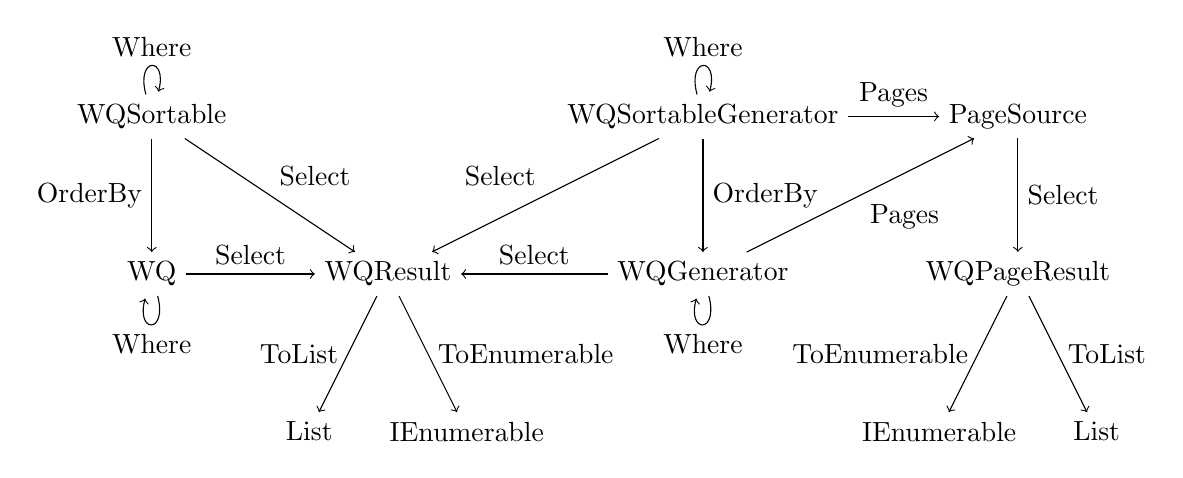
\begin{tikzpicture}
\path (2,4) node(WQS) {\lstinline{WQSortable}};
\path (2,2) node(WQ) {\lstinline{WQ}};

\path (5,2) node(WQR) {\lstinline{WQResult}};
\path (4,0) node(List) {\lstinline{List}};
\path (6,0) node(IE) {\lstinline{IEnumerable}};

\path (9,4) node(WQSG) {\lstinline{WQSortableGenerator}};
\path (9,2) node(WQG) {\lstinline{WQGenerator}};

\path (13,4) node(PS) {\lstinline{PageSource}};
\path (13,2) node(WQPR) {\lstinline{WQPageResult}};
\path (14,0) node(PList) {\lstinline{List}};
\path (12,0) node(PIE) {\lstinline{IEnumerable}};

\draw[->] (WQS) edge [loop above] node {\lstinline{Where}} ();
\draw[->] (WQS) edge node[left] {\lstinline{OrderBy}} (WQ);
\draw[->] (WQS) edge node[above right] {\lstinline{Select}} (WQR);

\draw[->] (WQ) edge [loop below] node {\lstinline{Where}} ();
\draw[->] (WQ) edge node[above] {\lstinline{Select}} (WQR);

\draw[->] (WQR) edge node[left] {\lstinline{ToList}} (List);
\draw[->] (WQR) edge node[right] {\lstinline{ToEnumerable}} (IE);

\draw[->] (WQSG) edge [loop above] node {\lstinline{Where}} ();
\draw[->] (WQSG) edge node[right] {\lstinline{OrderBy}} (WQG);
\draw[->] (WQSG) edge node[above left] {\lstinline{Select}} (WQR);

\draw[->] (WQG) edge [loop below] node {\lstinline{Where}} ();
\draw[->] (WQG) edge node[above] {\lstinline{Select}} (WQR);

\draw[->] (WQSG) edge node[auto] {\lstinline{Pages}} (PS);
\draw[->] (WQG) edge node[below right] {\lstinline{Pages}} (PS);

\draw[->] (PS) edge node[auto] {\lstinline{Select}} (WQPR);
\draw[->] (WQPR) edge node[right] {\lstinline{ToList}} (PList);
\draw[->] (WQPR) edge node[left] {\lstinline{ToEnumerable}} (PIE);

\end{tikzpicture}

\caption{TODO}
\label{WikiQuery types}

\end{figure}

% WikiQuery
% PageSources and types related to prop queries
% ExpressionParser
% QueryParameters
% QueryProcessor, its helpers

\subsection{\lstinline{Downloader}}

% TODO: reword
Probably the most basic type in this project is \lstinline{Downloader}.
It takes care of forming the query string, executing the request and
returning the result as an \lstinline{XDocument}.

\lstinline{XDocument} is part of LINQ to XML, a part of .Net framework for manipulating XML documents.

\lstinline{Downloader} always uses POST and formats its requests as \path{application/x-www-form-urlencoded}.
This means that all modules work, including those that require POST.
On the other hand, uploads of files don't work, because they require \path{multipart/form-data}.

The decision to use \path{application/x-www-form-urlencoded} follows from the fact that
\path{multipart/form-data} is very inefficient when sending multiple parameters with short values,
which is common when making requests to the API.

% TODO: maybe some conclusion?

\section{The LinqToWiki.Codegen project}

\section{The linqtowiki-codegen application}

\section{Samples of queries}